\documentclass{standalone}
\usepackage{tikz}
\usepackage{times}
\usepackage{amsmath}
\usepackage{txfonts}
\usepackage[utf8]{inputenc}
\usetikzlibrary{backgrounds}

\begin{document}
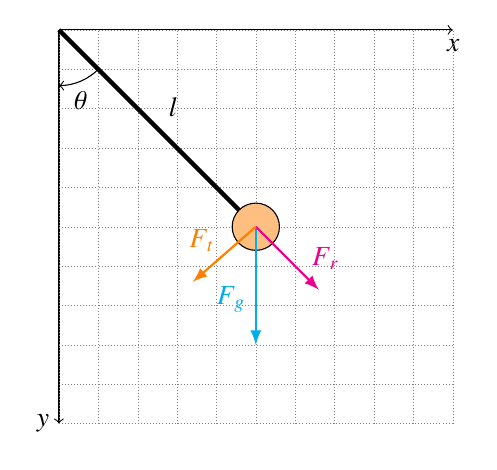
\begin{tikzpicture}
    
    % Koordinatensystem
    \def\pendulumorigin{0,0}

    \draw[->] (\pendulumorigin) -- ++(5,0) node[below] {$x$};
    \draw[->] (\pendulumorigin) -- ++(0,-5) node[left] {$y$};

    % Definition der Gitterparameter
    \def\rows{0} % Anzahl der Zeilen
    \def\cols{5} % Anzahl der Spalten
    \def\spacing{0.5} % Abstand zwischen den Linien

    \draw[step=\spacing,gray,densely dotted, ultra thin] (0,-5) 
    grid (\cols,\rows);

    % Koordinaten
    \coordinate (pivot) at (0,0);
    \coordinate (bob) at (2.5,-2.5);

    % Pendelstange
    \draw[ultra thick] (pivot) -- (bob) node[midway,above right] {$l$};

    % Masse
    \filldraw[fill=orange!50] (bob) circle (0.3);

    % Vektoren
    \draw[-latex,cyan,thick] (bob) -- ++(0,-1.5) node[midway,left,yshift=-5pt] {$F_g$}; % v1
    \draw[-latex,magenta,thick] (bob) -- ++(0.8,-0.8) node[midway,right,xshift=5pt] {$F_r$}; % v2
    \draw[-latex,orange,thick] (bob) -- ++(-0.8,-0.7) node[midway,left,yshift=5pt] {$F_t$}; % v1-v2

    % Winkel
    \def\xang{0.5} % x-Koordinate des Winkels
    \def\yang{-0.5} % y-Koordinate des Winkels

    % Zeichnen des Winkels
    \draw[->] (\xang,\yang) arc (-45:-90:0.707) node[midway,below] {$\theta$};

\end{tikzpicture}
\end{document}